\section{Practical Methods for Opacity Calculations$^\ddagger$}

In atmospheric retrieval, opacity calculations often dominate both accuracy and computational speed.  
Here, we introduce representative methods for opacity computation.

\subsection*{Direct Calculation}

The cross section of the $l$-th line of the $m$-th molecule can be expressed as
\begin{align}
  \sigma_{m,l}(\nu) &= S_{m,l} g_\mathrm{V}(\nu - \hat{\nu} , \beta, \gamma_L) \\
  &= \frac{S_{m,l}}{\sqrt{2 \pi} \beta} H\left( \frac{\nu -\hat{\nu}}{\sqrt{2} \beta},\frac{\gamma_L}{\sqrt{2} \beta} \right),
\end{align}
where $S_{m,l}$ is the line strength and $g_\mathrm{V}(\nu, \beta, \gamma_L)$ is the Voigt function.  
$\hat{\nu}$ is the line center. The Voigt function can be written as the convolution of a Lorentz profile and Doppler broadening:
\begin{align}
g_\mathrm{V}(\nu, \beta, \gamma_L) = g_\mathrm{L} (\nu,\gamma_L) \ast g_\mathrm{D} (\nu,\beta) 
\end{align}
where
\begin{align}
 g_\mathrm{L} (\nu,\gamma_L) &= \frac{\gamma_L/\pi}{\nu^2 + \gamma_L^2} \\
 g_\mathrm{D} (\nu,\beta) &= \mathcal{N} (0, \beta).
\end{align}

Note that $\beta$ is the standard deviation of Doppler broadening, with the relation $\beta = \gamma_D/\sqrt{2 \log{2}}$.  
The function $H(x,a)$ is the Voigt--Hjerting function \cite{1938ApJ....88..508H}, defined as
\begin{align}
H(x,a) = \frac{a}{\pi} \int_{-\infty}^{\infty} \frac{e^{-y^2}}{(x-y)^2 + a^2} dy.
\end{align}

The Voigt-Hjerting function is the real part of the Faddeeva function 
$w(z) = \exp{(-z^2)} \, \mathrm{erfc}(-i z)$ with $z = x + i a \in \mathbb{C}$:
\begin{align}
H(x,a) = \mathrm{Re}[w(x +i a)].
\end{align}

In Python, the Faddeeva function $w(z)$ is widely used through {\sf wofz} (``w of z''), 
which is based on Algorithm 680 of the {\it Transactions of Mathematical Software} \cite{poppe1990algorithm}.

As an alternative form of the Voigt--Hjerting function, the following formulation by Zaghloul and Ali \cite{2011arXiv1106.0151Z} is also frequently used:
\begin{align}
\label{eq:algo916}
\hat{H}_{\Ncut}(x,a) &= e^{-x^2} \mathrm{erfcx} (a) \cos{(2 x a)} \nonumber \\
&+ \frac{2 \eta x \sin{(a x)}}{\pi}  e^{-x^2} \mathrm{sinc} (a x/\pi) \nonumber \\
&+ \frac{2 \eta}{\pi} \left\{  - a \cos{(2 a x)} \Sigma_1 + \frac{a}{2} \Sigma_2 + \frac{a}{2} \Sigma_3 \right\},
\end{align}
where
\begin{align}
\Sigma_1 &= \sum_{n=1}^{\Ncut} \left( \frac{1}{\eta^2 n^2 + a^2}\right) e^{-(\eta^2 n^2 + x^2)}  \\
\Sigma_2 &= \sum_{n=1}^{\Ncut} \left( \frac{1}{\eta^2 n^2 + a^2}\right) e^{-(\eta n + x)^2}  \\
\Sigma_3 &= \sum_{n=1}^{\Ncut} \left( \frac{1}{\eta^2 n^2 + a^2}\right) e^{-(\eta n - x)^2}, 
\end{align}
and $\mathrm{erfcx} (x) = 2 \pi^{-1/2} e^{x^2} \int_x^\infty e^{-t^2} dt$ is the scaled complementary error function.  
$\eta \le 1$ is a control parameter, and $\eta=0.5$ is commonly adopted\footnote{When $M \to \infty$, the Voigt--Hjerting function is recovered. In practice, however, truncation at a suitable integer is necessary. The above expression approximates well for $|x| \lesssim \Ncut/2$, while for $|x| > \Ncut/2$ it rapidly approaches zero. In {\sf ExoJAX} \href{https://github.com/HajimeKawahara/exojax}{}, we adopt $\Ncut=27$, and for $|x|>\Ncut/2$ we use the asymptotic form of the Faddeeva function:
\begin{align}
\label{eq:asywofz}
  w_n^\mathrm{asy}(z) &= \frac{i}{z \sqrt{\pi}} \left( 1 + \tilde{\alpha} ( \mathsf{s}_0 + \tilde{\alpha} ( \mathsf{s}_1 +  \cdots \tilde{\alpha}  ( \mathsf{s}_n )\cdots) \right),
\end{align}
where $\tilde{\alpha} \equiv {1}/{2 z^2}$, and the real part is taken as a substitute.}.

\subsection*{Multi-Line Cross Section Synthesis via Discrete Integral Transform}

The method based on the Discrete Integral Transform (DIT) was proposed by van den Bekerom and Pannier \cite{van2021discrete} to efficiently compute the cross sections of a large number of lines.  
In the DIT approach, instead of summing over each absorption line directly, the calculation is reformulated as an integration in parameter space using the line-shape density (LSD), $\mathfrak{S}(\nulc,\beta,\gamma_L)$, and then discretized for evaluation. That is,
\begin{align}
\sigma (\nu) &= \sum_l S_l V(\nu - \nulc_l, \beta_l, \gamma_{L,l}) \\
&= \int d \nulc \int d \beta \int d \gamma_L  \mathfrak{S}(\nulc,\beta,\gamma_L) g_\mathrm{V}(\nu - \nulc, \beta, \gamma_{L})\\
&\approx \sum_{jhk} \mathfrak{S}_{jhk} g_\mathrm{V}(\nu_i - \nulc_j, \beta_h, \gamma_{L,k}) 
\label{eq:FTFT}
\end{align}

In the original DIT, each line is stored in the three-dimensional grid 
$\mathfrak{S} (\nu_j, \beta_h,\gamma_{L,k})$ weighted by its line strength.  
Here, the Voigt function can be expressed as
\begin{align}
\sigma (\nu_i) &= \sum_{hk} \mathrm{FT}^{-1} [ \mathrm{FT} (\mathfrak{S}_{jhk})  \mathrm{FT} (g_\mathrm{V} (\nulc_j, \beta_h, \gamma_{L,k})) ] \\
\sigma (\nu_i) &= \sum_{hk} \mathrm{FT}^{-1} [ \mathrm{FT} (\mathfrak{S}_{jhk})  \mathrm{FT} (g_\mathrm{D} ) \mathrm{FT} (g_\mathrm{L})] 
\end{align}
where the Fourier transforms of $g_D$ and $g_L$ are written simply as
\begin{align}
\mathrm{FT} (g_\mathrm{D} ) &= e^{-2 (\pi \beta k)^2 }\\
\mathrm{FT} (g_\mathrm{L})  &= e^{-2 \pi \gamma_L |k| }.
\end{align}

Although omitted here, since DIT relies on Fourier transforms, it is necessary to take care to avoid aliasing effects\footnote{DIT uses a grid in wavenumber space, but in astronomical applications it is more convenient to adopt a logarithmic wavenumber grid, which naturally incorporates radial velocity shifts. In this case, when temperature is fixed, the Doppler width for the same isotope becomes universal across lines, allowing the LSD dimension to be reduced by one. This modified version of DIT is called MODIT.}.

\subsection*{Correlated $k$-Distribution Method}

The correlated $k$-distribution method (CKD) traces back to the 1960s, when Malkmus introduced the probability distribution of absorption coefficients and proposed the $k$-distribution method to average molecular band absorption \cite{malkmus1967random}.  
Later, in 1989, Goody et al. introduced the idea of rearranging $k$ values so that spectral ordering is preserved even in vertically inhomogeneous atmospheres, which became the core of the ``correlated'' $k$-distribution method \cite{1989JQSRT..42..539G}.  
In 1991, Lacis \& Oinas organized its implementation into the radiative transfer equation and verified its accuracy, establishing it as a standard technique in climate models and planetary atmosphere calculations \cite{1991JGR....96.9027L}.  
Good references on correlated $k$-distributions include \cite{liou2002introduction}.

\subsection*{$k$-Distribution}

\begin{figure*}[b]
    \centering
    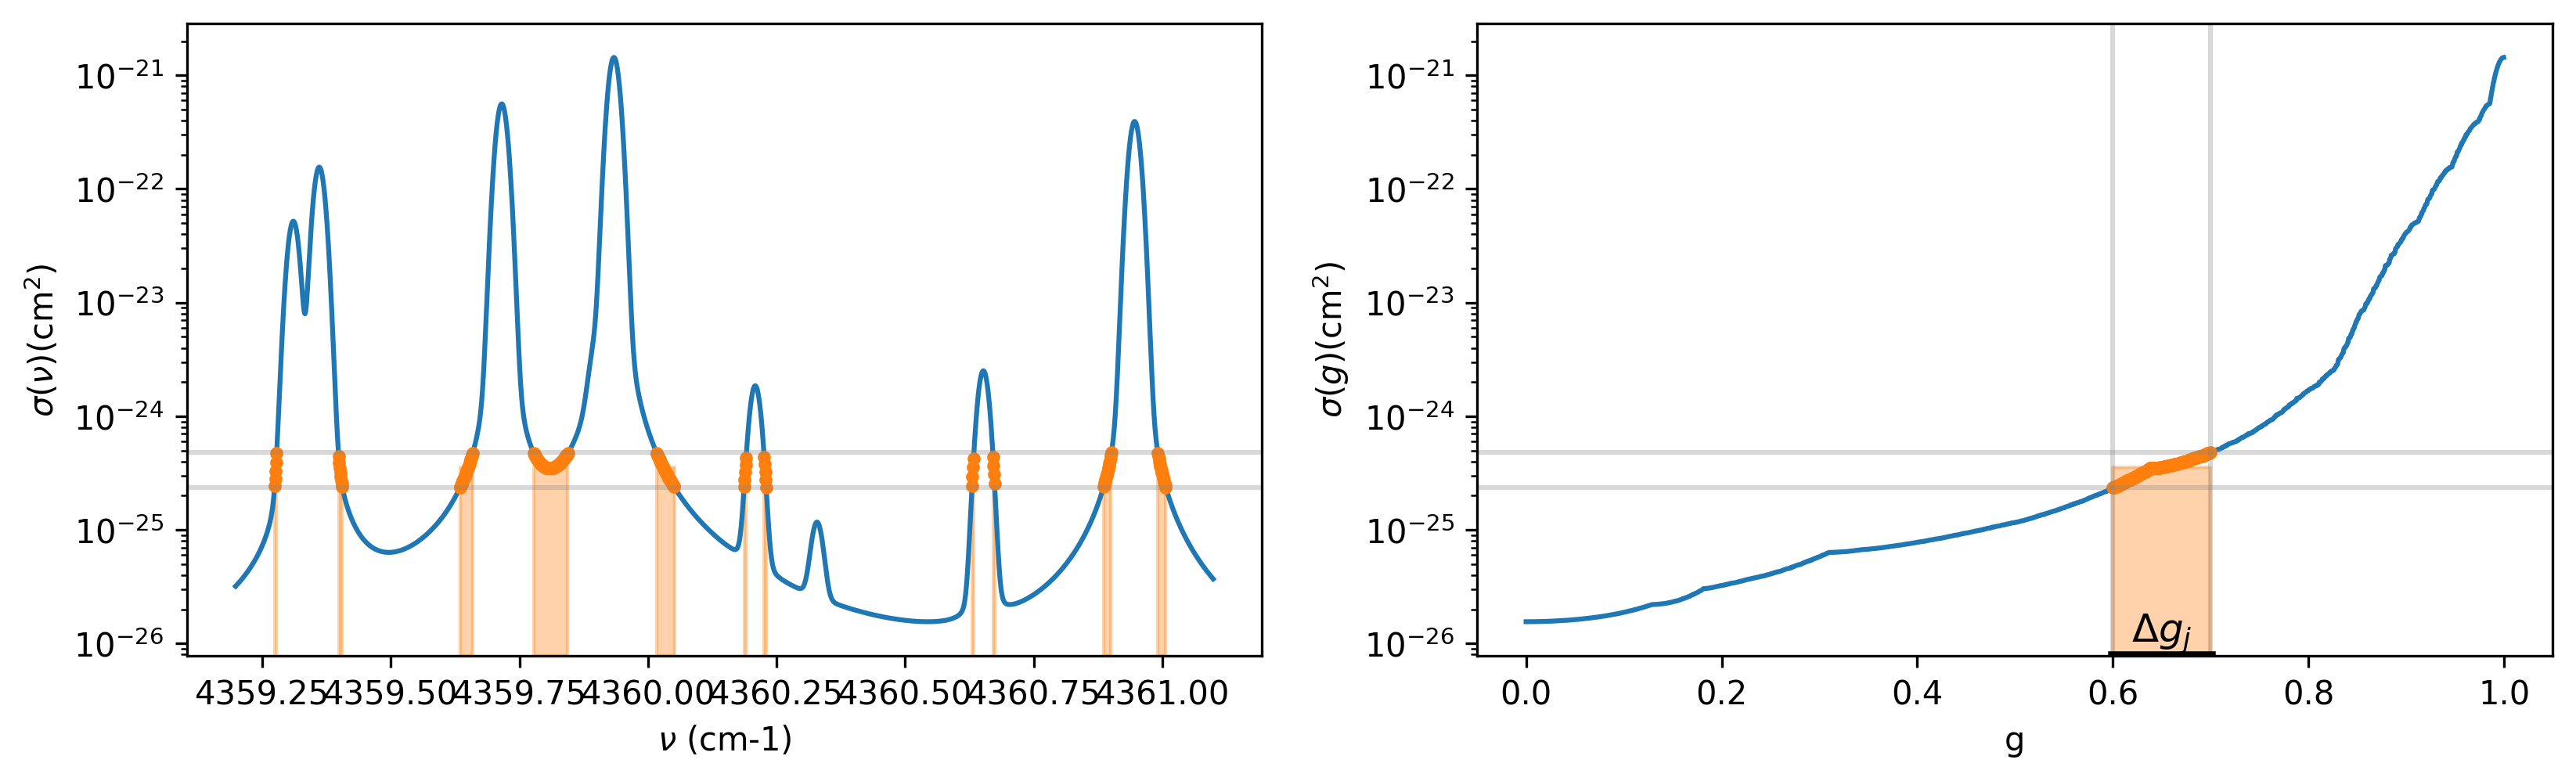
\includegraphics[width=1.0\linewidth]{fig/ckd/corrk_test.png}
    \caption{Left: Cross section of water shown in wavenumber space. Right: The same cross section represented in $g$-space. The orange region corresponds to the cross section belonging to the interval $g=0.6-0.7$ ($\Delta g_i$) in $g$-space.}
    \label{fig:ckd_fig1}
\end{figure*}

The cross section $\sigma(\nu)$ (or opacity), when viewed over a spectral region broader than the line width, is a non-injective function. That is, there exist multiple $\nu$ values corresponding to the same $\sigma^\prime = \sigma(\nu)$ (Fig.~\ref{fig:ckd_fig1}, left).  
This non-injectivity increases as the wavelength range broadens.  
Therefore, it is natural to consider describing the information not in terms of $\nu$, but in terms of the values of $\sigma$.  

For example, consider integrating a nonnegative function $f(\sigma(\nu)) \geq 0$ over some wavenumber range.  
In a Riemann integral this is written as
\begin{align}
 I &= \int_\mathrm{min}^\mathrm{max} f(\sigma(\nu)) d \nu \approx  \sum_i f(\sigma(\nu_i)) \Delta \nu_i.
\end{align}
Here, the integration domain is divided in the $\nu$ direction.  
However, as non-injectivity increases, one must sum over the same $\sigma$ values many times.  
Thus, it is useful to consider integration with respect to the measure of the range instead.

Now, divide the range into disjoint sets.  
Let $A_j$ be the set of $\nu$ values whose range lies within a small region $\Delta \sigma$ around $\sigma = \sigma_j$.  
The range can then be expressed as
\begin{align}
    V = \bigcup_{j=0}^{n} A_j.
\end{align}

Using the characteristic function of set $A$,
\begin{align}
   \chi_A (\nu) &= \begin{cases}
  1, & \text{if } \nu \in A \\
  0, & \text{if } \nu \notin A,
\end{cases}
\end{align}
we consider the (nonnegative) simple function
\begin{align}
    s(\nu) = \sum_j^n f_j \chi_{A_j}(\nu),
\end{align}
where $0 \leq f_0 < f_1 < \cdots < f_n$.  
The Lebesgue integral is defined as
\begin{align}
    \int_V s(\nu) d \nu = \sum_{j=0}^n f_j \, m_d (A_j),
\end{align}
where $m_d(A_j)$ is the measure of $A_j$.  
Applying this idea, we divide the range into bins from minimum to maximum and index them as $j=0,1,\cdots$, assigning representative values $\sigma_j$.  
Approximating $f(\sigma(\nu))$ by a simple function,
\begin{align}
    f(\sigma(\nu)) \approx s(\nu) = \sum_j^n f(\sigma_j) \chi_{A_j}(\nu),
\end{align}
we obtain
\begin{align}
 \int_V f(\sigma(\nu)) d \nu &\approx \int_V s(\nu) d \nu = \sum_j f(\sigma_j) \Delta m_j \\
 &= (\nu_\mathrm{max} - \nu_\mathrm{min}) \sum_j f(\sigma_j) \Delta g_j,
\end{align}
where $\Delta m_j = (\nu_\mathrm{max} - \nu_\mathrm{min}) \Delta g_j$ is the measure of each set.  

The final expression can be viewed as an approximation to the (Riemann) integral
\begin{align}
(\nu_\mathrm{max} - \nu_\mathrm{min}) \int_0^1 f(\sigma(g)) dg,
\end{align}
and becomes exact in the limit of infinite refinement:
\begin{align}
\label{eq:Lebesgue}
\int_V f(\sigma(\nu)) d \nu = (\nu_\mathrm{max} - \nu_\mathrm{min}) \int_0^1 f(\sigma(g)) dg.
\end{align}

Here, $\sigma_j$ corresponds to bins taken from smaller to larger values, and $\Delta m_j$ represents the measure of the domain corresponding to these bins, i.e., the length of the $\nu$ space.  
Practically, $\sigma(g)$ is obtained by sorting a finely sampled table of $\sigma(\nu)$ and normalizing it to $[0,1]$.  
Figure~\ref{fig:ckd_fig1} (right) shows $\sigma(g)$ obtained in this way—essentially the cumulative distribution function of $\sigma$.  
Since it is based on sorting, it is a monotonically increasing function.  
The name ``$k$-distribution'' originates from using opacity (commonly denoted $k$) in this distribution function.

The shaded regions in Fig.~\ref{fig:ckd_fig1} illustrate the contribution from $\Delta g_j$ when $f(\sigma) = \sigma$, shown in $\nu$-$f$ space (left) and $g$-$f$ space (right).  
In the left panel, $\Delta m_j$ corresponds to the sum of the shaded lengths along the $\nu$ axis.  
Dividing by $(\nu_\mathrm{max} - \nu_\mathrm{min})$ yields $\Delta g_j$, shown in the right panel.

Once $\sigma(g)$ is obtained by sorting, the evaluation of the right-hand side of Eq.~(\ref{eq:Lebesgue}) can be performed using standard numerical integration methods such as Gauss-Legendre quadrature.

\begin{figure*}[!h]
    \centering
    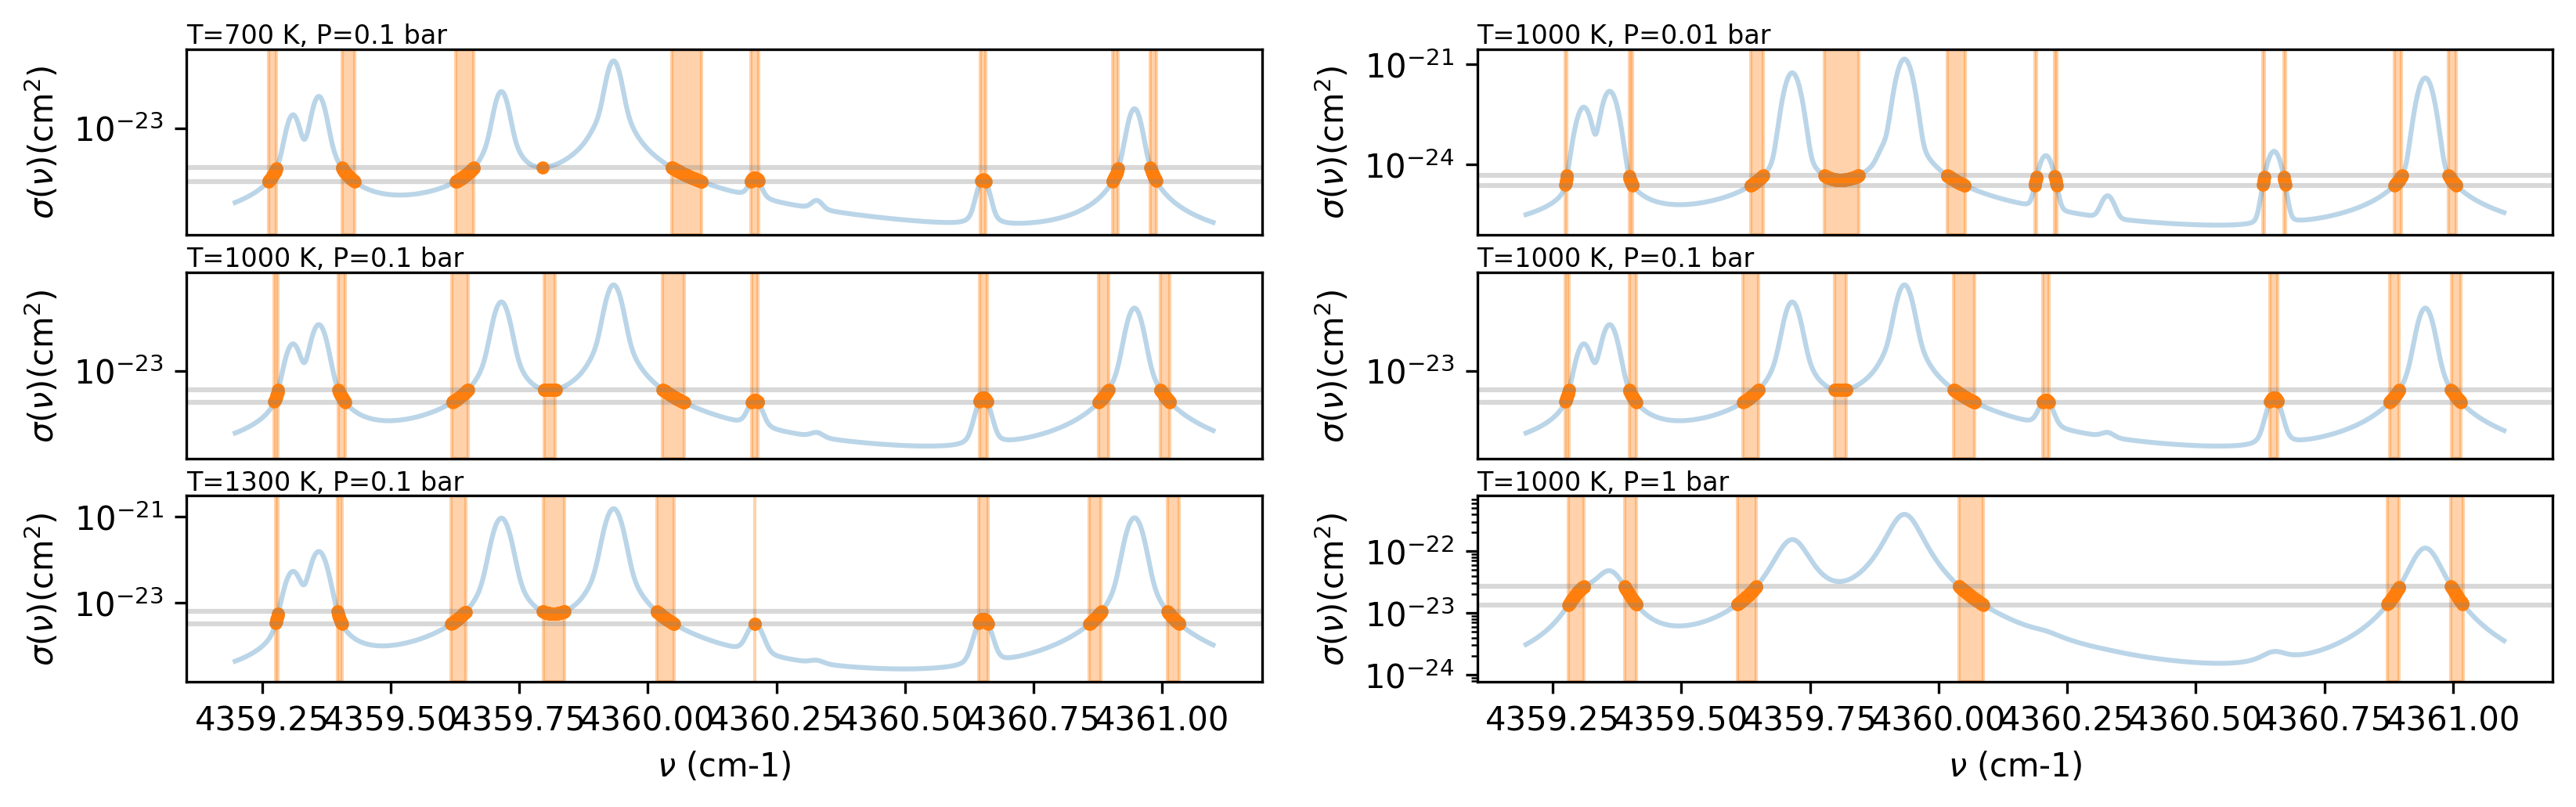
\includegraphics[width=1.0\linewidth]{fig/ckd/corrk_corr.png}
    \caption{Left: Cross sections in $g$-space corresponding to $g=0.6-0.7$ ($\Delta g_i$) are shown in orange when temperature is varied between 700, 1000, and 1300 K at $p=0.1$ bar. The same $\Delta g_i$ as in Fig.~\ref{fig:ckd_fig1} is adopted. Right: Cross sections corresponding to the same $\Delta g_i$ are shown in orange when temperature is fixed at 1000 K and pressure is varied between 0.01, 0.1, and 1 bar.}
    \label{fig:ckd_fig2}
\end{figure*}

So far we considered a single-layer integral, but in radiative transfer the opacity differs layer by layer, and integration must be performed over wavenumber.  
If this can be replaced by integration over sets $\Delta g_j$, significant computational savings are possible in highly non-injective cases.  
In other words, the orange regions in the left panel of Eq.~(\ref{eq:Lebesgue}) can be grouped as having similar opacity, allowing radiative transfer to be solved collectively.  

However, this requires that the $\nu$ sets corresponding to $\Delta g_j$ be identical across layers.  
Such an assumption is called comonotonicity: if the ordering of $\nu$ remains consistent when sorted by range ($\sigma$), then it holds regardless of how $\Delta g_j$ is chosen.  
The ``correlation'' in the correlated $k$-distribution method refers to this assumption of comonotonicity between layers.  
In terms of copulas, this is equivalent to assuming the Fréchet -- Hoeffding upper bound.

Figure~\ref{fig:ckd_fig2} illustrates $\Delta g_j$ under varying temperature and pressure.  
As seen in this example, while the sets align well around the line centers, the agreement worsens in the wings.
